%
% einstrahlung.tex
%
% (c) 2018 Prof Dr Andreas Müller,Hochschule Rapperswil
%
\subsection{Einstrahlung auf einen Breitenkreis}
Wir berechnen die Einstrahlung auf einem gegebenen Breitengrad
$\vartheta$ in Abhängigkeit von der Neigung $\gamma$
der Erdachse.
Die einfallende Strahlungsleistung ist proportional zum Skalarprodukt
der Richtung der Einstrahlung mit der Normalen in einem Punkte
auf dem Breitenkreis zur Breite $\vartheta$.
Die Normale ist
\[
\vec n(\vartheta,\varphi)
=
\begin{pmatrix}
\sin\vartheta\cos\varphi\\
\sin\vartheta\sin\varphi\\
\cos\vartheta
\end{pmatrix}.
\]
Die Richtung der Einstrahlungsrichtung ist
\[
\vec e(\gamma)
=
\begin{pmatrix}
\cos\gamma\\
0\\
\sin\gamma
\end{pmatrix}.
\]
Das Skalarprodukt ist
\begin{equation}
\vec n(\vartheta,\varphi)\cdot\vec e(\gamma)
=
\sin\vartheta\cos\varphi\cos\gamma
+
\cos\vartheta\sin\gamma.
\label{skript:einstrahlung:skalarprodukt}
\end{equation}
Für die folgende Diskussion nehmen wir an, dass $\gamma >= 0$,
dass also der Nordpol permanent bestrahlt ist und der Südpol keine
Strahlung erhält.

Im Folgenden wollen wir die Energie berechnen, die in eine Zone
eingestrahlt wird.

\subsubsection{Sonnenauf- und -untergang}
Die Einstrahlung erfolgt natürlich nur zwischen Sonnenauf- und
-untergang.
Wir bezeichen die geographische Länge, bei der der Sonnenauf- oder
-untergang erfolgt, mit $\pm\varphi_0$.
Diese sind gekennzeichnet dadurch, dass $\vec n(\vartheta,\varphi_0)$ und
$\vec e(\gamma)$ senkrecht aufeinander stehen oder
\begin{equation*}
\begin{aligned}
&&
\vec n(\vartheta,\varphi_0)&\perp \vec e(\gamma)
\\
&\Rightarrow&
\vec n(\vartheta,\varphi_0)\cdot \vec e(\gamma)&=0
\\
&\Rightarrow&
\sin\vartheta\cos\varphi_0\cos\gamma
&=
-
\cos\vartheta\sin\gamma
\\
&\Rightarrow&
\cos\varphi_0
&=
-\frac{\tan\gamma}{\tan\vartheta}.
\end{aligned}
\end{equation*}
Wenn $\vartheta < \gamma$ (Punkt in der Nähe des Nordpols) oder
$\vartheta > \pi - \gamma$ (Punkt in der Nähe des Südpols),
dann hat die Gleichung keine Lösung,
die Sonne geht nie auf (Polarnacht) oder unter (Polartag).

\subsubsection{Mittlere Strahlungsleistung auf Breite $\vartheta$}
Um die Strahlungsleistung auf einer beliebigen geographischen
Breite zu berechnen, gehen wir in zwei Schritten vor.
Das Skalarprodukt~\eqref{skript:einstrahlung:skalarprodukt} 
gibt die Strahlungsleistung $\varepsilon(\vartheta,\varphi,\gamma)$
in einem Punkt auf der geographischen
Breite $\vartheta$ in Abhängigkeit von $\varphi$.
Im ersten Schritt mitteln wir dies über eine Umdrehung, dazu
ist das Skalarprodukt~\eqref{skript:einstrahlung:skalarprodukt} über eine
Umdrehung zu mitteln.
So erhalten wir die mittlere Strahlungsleistung $\varepsilon(\vartheta,\gamma)$
in einem Punkte auf geographischer Breite $\vartheta$.
Im zweiten Schritt müssen wir die die mittlere Strahlungsleistung mit
der Länge des Breitenkreises multiplizieren, um die Strahlungsleistung
auf dem Breitenkreis zur Breite $\vartheta$ zu erhalten.

\subsubsection{Polnähe}
In der Nähe des Südpols, also wenn $\vartheta > \pi - \gamma$,
ist die Einstrahlung $=0$.
In der Nähe des Nordpols, also wenn $\vartheta < \gamma$, ist die
Einstrahlungsdichte
\[
\varepsilon_{\text{in}}
=
\int_0^{2\pi}
\sin\vartheta\cos\varphi\cos\gamma
+
\cos\vartheta\sin\gamma
\,d\varphi
=
2\pi\cos\vartheta\sin\gamma.
\]
Für den Spezialfall $\vartheta=0$ fällt der erste Term weg und es
bleibt 
\begin{align*}
\varepsilon_{\text{in}}(0,\gamma)
&=
2\pi\sin\gamma.
\end{align*}

\subsubsection{Äquator}
Am Äquator ist $\vartheta=\frac{\pi}2$ und $\varphi_0=\frac{\pi}2$.
Man bekommt
\begin{align*}
\varepsilon_{\text{in}}\biggl(\frac{\pi}2,\gamma\biggr)
&=
\int_{-\varphi_0}^{\varphi_0}
\cos\varphi\cos\gamma\,d\varphi
=
\cos\gamma
\int_{-\frac{\pi}2}^{\frac{\pi}2}
\cos\varphi
\,d\varphi
=
2\cos\gamma
\end{align*}
für die Einstrahlung am Äquator.

\subsubsection{Der allgemeine Fall mit Sonnenauf- und -untergang}
\begin{figure}
\centering
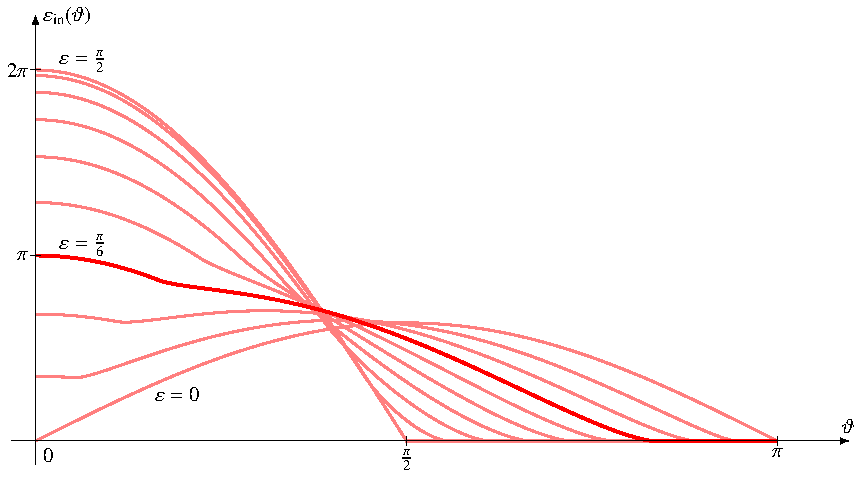
\includegraphics[width=\hsize]{chapters/5/ein.pdf}
\caption{Über eine Rotation gemittelte Einstrahlungsdichte
in Abhängigkeit von der geographischen Breite
gemäss Formel~\eqref{skript:einstrahlung:plottable} für verschiedene
Neigungen $\gamma$ der Achse. 
Dargestellt sind $\gamma$-Werte zwischen 0 und $90^\circ$ 
in $10^\circ$-Schritten. 
Die Neigung $\gamma=30^\circ=\frac{\pi}{6}$ ist hervorgehoben.
\label{skript:einstrahlung:ein}}
\end{figure}%
Der allgemeine Fall mit Sonnenauf- und -untergang
ist $\gamma < \vartheta < \pi-\gamma$.
Für die Einstrahlung finden wir dann
\begin{align}
\varepsilon_{\text{in}}(\vartheta,\gamma)
&=
\int_{-\varphi_0}^{\varphi_0}
\sin\vartheta\cos\varphi\cos\gamma
+
\cos\vartheta\sin\gamma\,d\varphi
\notag
\\
&=
\sin\vartheta\cos\gamma\biggl[\sin\varphi\biggr]_{-\varphi_0}^{\varphi_0}
+
2\varphi_0 \cos\vartheta\sin\gamma
\notag
\\
&=
2\sin\vartheta\cos\gamma\sin\varphi_0
+
2\varphi_0 \cos\vartheta\sin\gamma
\notag
\\
&=
2\sin\vartheta\cos\gamma
\sin
\arccos\biggl(-\frac{\tan\gamma}{\tan\vartheta}\biggr)
+
2\cos\vartheta\sin\gamma
\arccos\biggl(-\frac{\tan\gamma}{\tan\vartheta}\biggr).
\notag
\\
\intertext{Im ersten Term können wir $\sin\arccos x  = \sqrt{1-x^2}$
verwenden.
Den zweiten Term könnten wir so stehen lassen, aber für die graphische
Darstellung brauchen wir eine Darstellung das Arkuskosinus durch den
Arkustangens, da TikZ nur den Arkustangens anbietet.
Wir verwenden die Formel $\arccos x = 2\arctan\sqrt{(1-x)/(1+x)}$ und
erhalten}
&=
2\sin\vartheta\cos\gamma
\sqrt{1-\frac{\tan^2\gamma}{\tan^2\vartheta}}
+
4\cos\vartheta\sin\gamma
\arctan\sqrt{\frac{1+\frac{\tan\gamma}{\tan\vartheta}}{1-\frac{\tan\gamma}{\tan\vartheta}}}
\notag
\\
&=
\pm2\cos\vartheta\cos\gamma
\sqrt{\tan^2\vartheta-\tan^2\gamma}
+
4\cos\vartheta\sin\gamma
\arctan\sqrt{\frac{\tan\vartheta+\tan\gamma}{\tan\vartheta-\tan\gamma}}
\notag
\\
&=
2
\cos\vartheta
\biggl(
\cos\gamma
\sqrt{\frac{\tan^2\vartheta}{\tan^2\gamma}-1}
+
2
\sin\gamma
\arctan\sqrt{
\frac{\tan\vartheta+\tan\gamma}{\tan\vartheta-\tan\gamma}
}
\biggr).
\label{skript:einstrahlung:plottable}
\end{align}
Formel~\eqref{skript:einstrahlung:plottable} ist in
Abbildung~\ref{skript:einstrahlung:ein} dargestellt.

\subsubsection{Strahlungsleistung auf dem Breitenkreis $\vartheta$}
\begin{figure}
\centering
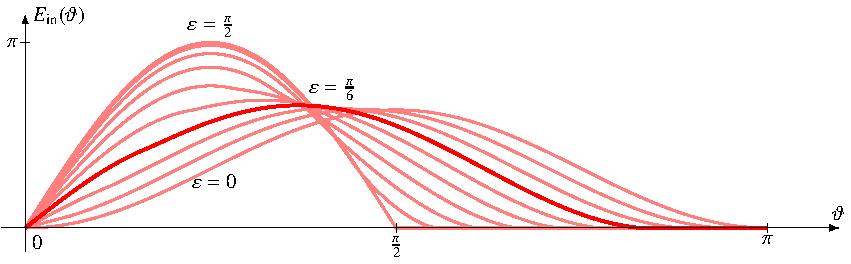
\includegraphics[width=\hsize]{chapters/5/ein1.pdf}
\caption{Strahlungsleistung auf geographischer Breite $\vartheta$,
gegeben durch Formel~\eqref{skript:einstrahlung:breite}.
\label{skript:einstrahlung:ein1}}
\end{figure}%
Die gesamte Strahlungsleistung auf dem Breitenkreis $\vartheta$
ist
\begin{equation}
E_{\text{in}}(\vartheta)
=
\varepsilon(\vartheta,\gamma)
\cdot
\sin\vartheta
\label{skript:einstrahlung:breite}
\end{equation}
Die resultierende Funktion ist in Abbildung~\ref{skript:einstrahlung:ein1}
dargestellt.

%\subsection{Einstrahlung über ein Jahr}
%\begin{figure}
%\centering
%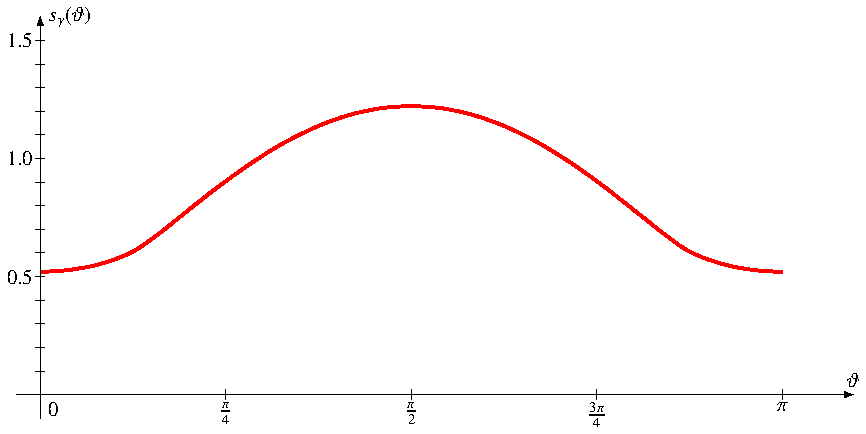
\includegraphics[width=\hsize]{chapters/5/total.pdf}
%\caption{Einstrahlung über ein Jahr in Abhängigkeit von der geographischen
%Breite.
%\label{skript:einstrahlung:total}}
%\end{figure}
%Die in \eqref{skript:einstrahlung:breite} gefunden Einstrahlung auf einem
%Breitengrad $\vartheta$ geht von einer konstanten Neigung der Erdachse aus.
%Die Bewegung der Erde um die Sonne bedeutet aber, dass die Neigung der
%der Erdachse scheinbar variert,
%es gilt nämlich
%\[
%\tan \gamma(t) = \tan\gamma_\text{max}\cdot \sin t.
%\]
%Für ein Klimamodell wesentlich ist daher der Mittelwert
%\[
%s_{\gamma_\text{max}}(\vartheta)
%=
%\frac1{2\pi}
%\int_0^{2\pi} \varepsilon(\vartheta,\gamma(t))\,dt
%\]
%von \eqref{skript:einstrahlung:breite} über ein Jahr.
%Abbildung~\ref{skript:einstrahlung:total} zeigt das Resultat der 
%numerischen Integration.

%
% jahr.tex
%
% (c) 2018 Prof Dr Andreas Müller, Hochschule Rapperswil
%
\subsection{Einstrahlung über ein Jahr}
Wir könnten versuchen, die im letzten Abschnitt gefundene Einstrahlung
über einen Tag über ein Jahr zu mitteln.
Allerdings stellt sich dies als nur schwer durchführbar heraus.
Stattdessen wählen wir ein Vorgehen, welches  sich an die 
noch etwas allgmeinere Untersuchung in 
\cite[section 5]{skript:mcgeheelehman}
anlehnt.
Dazu berechnen wir erst die mittlere Insolation auf eine nicht
rotierende und nicht geneigte Kugel im Laufe eines Jahres und
mitteln erst danach über den Tagesgang.

\subsubsection{Nicht drehende Erde}
\begin{figure}%
\centering%
\begin{tikzpicture}[>=latex,thick]
\node at (0,0) {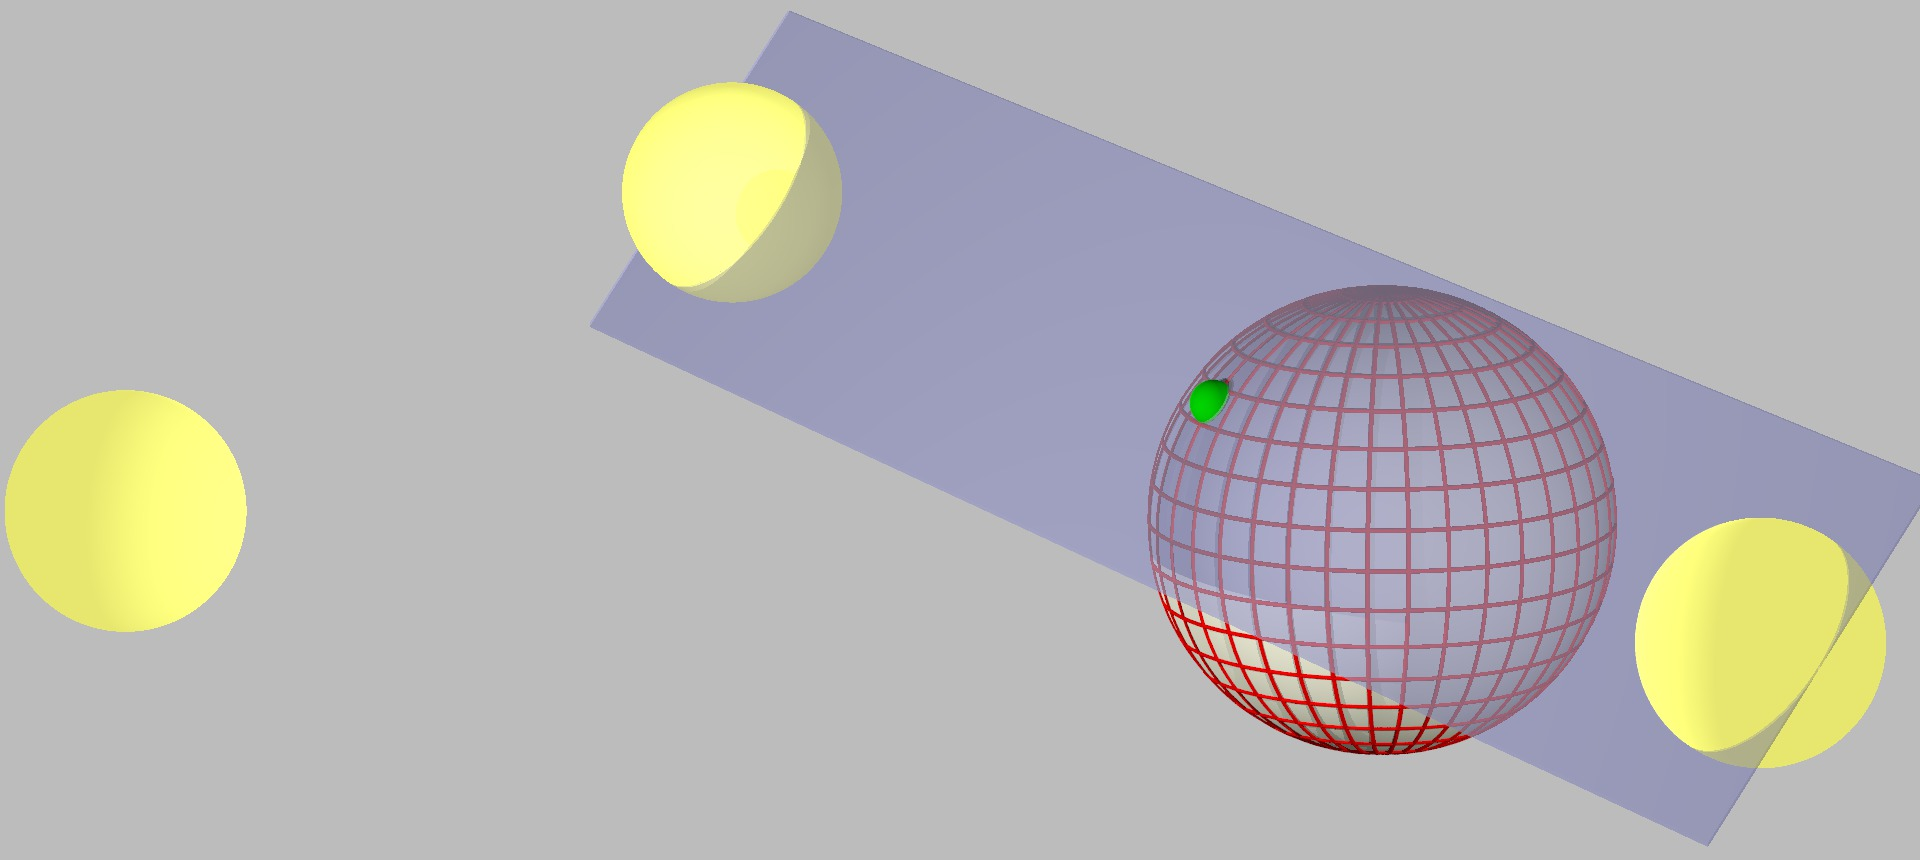
\includegraphics[width=\hsize]{chapters/5/midday.jpg}};
\end{tikzpicture}
\caption{Insolation eines Punktes auf einer nicht geneigten 
und nicht rotierenden Erde im Laufe eines Jahres.
\label{skript:insolation:fest}}
\end{figure}%
Wir betrachten zunächst eine die Sonne auf einer Kreisbahn mit Radius $r$
umlaufende Kugel vom Radius $R$, die sich nicht dreht und gegen die Bahn
nicht geneigt ist.
Wir bezeichnen die Kugel-Koordinaten auf dieser Kugel mit $\hat\vartheta$
und $\hat\varphi$ und wollen die mittlere Insolation
$I(\hat\vartheta,\hat\varphi)$ am Punkt $(\hat\vartheta,\hat\varphi)$
im Laufe eines Jahres berechnen.
Wir nehmen dabei an, dass die Sonne viel weiter entfernt ist als $R$,
also $R\ll r$.
Die Parallaxe des Punktes $(\hat\vartheta,\hat\varphi)$ ist daher
vernachlässigbar.
Da wir ausserdem vo einer Kreisbahn ausgehen, ist das Problem
rotationssymmetrisch um die $z$-Achse, wir können daher annehmen, dass
der Punkt $(\hat\vartheta,\hat\varphi)$ auf dem Nullmeridian liegt,
dass also $\hat\varphi=0$.

Statt die Kugel um die Sonne zu bewegen, können wir die Sonne auch
im Laufe eines Jahres gleichmässig um den Punkt $(\hat\vartheta,\hat\varphi)$
bewegen.
Wir drücken dies dadurch aus, dass der Punkt Strahlung aus der Richtung
$(\cos\lambda,\sin\lambda,0)$ erhält, $\lambda$ ist die Länge der Position
der Sonne.
Natürlich erhält der Punkt nur Strahlung, wenn die Sonne über dem lokalen
Horizont ist.
Für einen Punkt auf dem Nullmeridian bedeutet dies, dass
$-\frac{\pi}2\le \lambda \le \frac{\pi}2$ sein muss.
Diese Situation ist in Abbildung~\ref{skript:insolation:fest} 
dargestellt.

Die mittlere Insolation auf den Punkt $(\hat\vartheta,0)$ ist dann
\begin{align*}
I(\hat\varphi,0)
=
\frac{S_0}{2\pi}
\int_{-\frac{\pi}2}^{\frac{\pi}2}
\begin{pmatrix}
\cos\lambda\\\sin\lambda\\0
\end{pmatrix}
\cdot
\begin{pmatrix}
\sin\hat\vartheta\\0\\\cos\hat\vartheta
\end{pmatrix}
\,d\lambda
=
\frac{S_0}{2\pi}
\int_{-\frac{\pi}2}^{\frac{\pi}2}
\cos\lambda\sin\hat\vartheta\,d\lambda
=
\frac{S_0}{\pi} \sin\hat\vartheta.
\end{align*}
Darin ist $S_0$ der Strahlungsfluss ausserhalb der Erdatmosphäre.
Offenbar hängt die Insolation nur von $\sin\hat\vartheta$ ab.
Wir können dies auch durch die $z$-Koordinate ausdrücken, es
ist nämlich
\begin{equation}
\sin\hat\vartheta = \sqrt{1-\cos^2\hat\vartheta}=\sqrt{1-z^2}.
\label{skript:einstrahlung:sintheta}
\end{equation}

\subsubsection{Geneigte Erde}
Um die Insolation auf einen Punkt auf der geneigten Erde zu ermitteln
brauchen wir die Umrechnung von Koordinaten $(\vartheta,\varphi)$ 
in die geographische Breite in dem Koordinatensystem, welches im
vorangegangenen Abschnitt als Basis diente.
Die Drehmatrix
\[
D_\gamma
=
\begin{pmatrix}
\cos\gamma&0&-\sin\gamma\\
0&1&0\\
\sin\gamma&0&\cos\gamma
\end{pmatrix}
\]
dreht einen Punkt auf der Kugeloberfläche um den Neigungswinkel
$\gamma$ der Erde.
Wir erhalten für den Punkt $(\vartheta,\varphi)$
\[
D_\gamma\begin{pmatrix}
\sin\vartheta\cos\varphi\\
\sin\vartheta\sin\varphi\\
\cos\vartheta
\end{pmatrix}
=
\begin{pmatrix}
\cos\gamma\sin\vartheta\cos\varphi -\sin\gamma\cos\vartheta\\
\sin\vartheta\sin\varphi\\
\sin\gamma\sin\vartheta\cos\varphi + \cos\gamma\cos\vartheta
\end{pmatrix}.
\]
Davon brauchen wir nur die letzte Koordinate, es ist
\begin{equation}
\cos\hat\vartheta
=
\sin\gamma\sin\vartheta\cos\varphi+\cos\gamma\cos\vartheta.
\end{equation}
Auf der nicht rotierenden aber geneigten Erde ist die Insolation
im Punkt $(\vartheta,\varphi)$ also
\begin{equation}
I(\vartheta,\varphi)
=
\frac{S_0}{\pi}
\sin\hat\vartheta
=
\frac{S_0}{\pi}
\sqrt{1-
(\sin\gamma\sin\vartheta\cos\varphi+\cos\gamma\cos\vartheta)^2}.
\label{skript:chapter:inspunkt}
\end{equation}

\subsubsection{Mittelung über einen Tag}
\begin{figure}
\centering
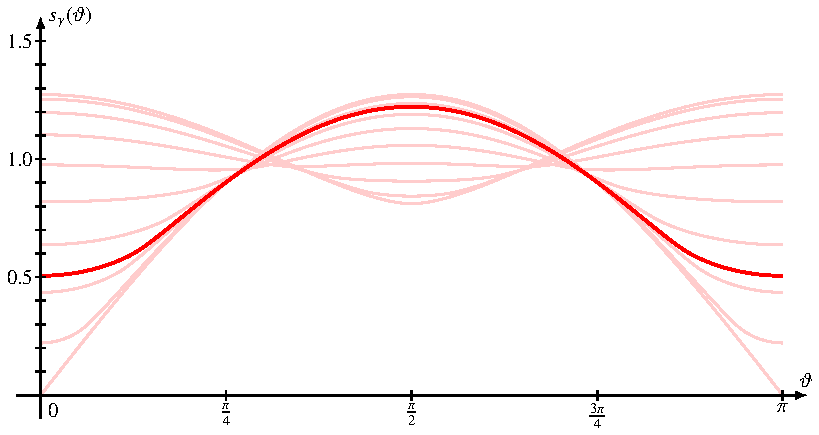
\includegraphics{chapters/5/ell2.pdf}
\caption{Mittlere Insolation über ein Jahr in Abhängigkeit von der
geographischen Breite.
Die hellroten Kurven zeigen die Insolation für Achsneigungen zwischen
$0^\circ$ ($\sin\theta$-Kurve mit Nullstellen an den Intervallenden)
und $90^\circ$.
\label{skript:einstrahlung:jahrinsbild}}
\end{figure}
Jetzt müssen wir die Insolation noch über die Rotation im Laufe eines 
Tages mitteln.
Wir erreichen dies, indem wir \eqref{skript:chapter:inspunkt}
über $\varphi$ über eine volle Umdrehung mitteln:
\begin{align*}
I(\vartheta)
&=
\frac{1}{2\pi}
\int_0^{2\pi}
\frac{S_0}{\pi}
\sqrt{1-
(\sin\gamma\sin\vartheta\cos\varphi+\cos\gamma\cos\vartheta)^2}
\,d\varphi
\\
&=
\frac{S_0}{2\pi^2}
\int_0^{2\pi}
\sqrt{1-
(\sin\gamma\sin\vartheta\cos\varphi+\cos\gamma\cos\vartheta)^2}
\,d\varphi.
\label{skript:einstrahlung:mittlereinsolation}
\end{align*}
Das Integral auf der rechten Seite ist nicht in geschlossener
Form lösbar.
Die numerische Berechnung mit Octave ergibt den Graphen
in Abbildung~\ref{skript:einstrahlung:jahrinsbild}.

Als Spezialfall sei notiert, dass im Falle verschwindender Neigung
$\gamma=0$ das Integral zu
\begin{align*}
I(\vartheta)
&=
\frac{S_0}{2\pi^2}
\int_{-\frac{\pi}2}^{\frac{\pi}2}
\sqrt{1-\cos^2\vartheta}
\,d\varphi
=
\frac{S_0}{2\pi^2}
\int_{-\frac{\pi}2}^{\frac{\pi}2}
\sin\vartheta
\,d\varphi
=
\frac{S_0}{\pi}
\sin\vartheta
\end{align*}
wird.
In Abbildung~\ref{skript:einstrahlung:jahrinsbild} ist dies die
Kurve mit den Nullstellen an den Intervalenden.
Man erkennt auch, dass im Spezialfall $\gamma=90^\circ$ die Insolation zu
\begin{align*}
I(\vartheta)
&=
\frac{S_0}{2\pi^2}
\int_{-\frac{\pi}2}^{\frac{\pi}2}
\sqrt{1- \sin^2\vartheta\cos^2\varphi}
\,d\varphi
\end{align*}
wird.
Man kann ablesen und sieht dies auch in der 
Abbildung~\ref{skript:einstrahlung:jahrinsbild} bestätigt, dass
die mittlere Insolation am Äquator ist als an den Polen.
Wenn nämlich $\sin\vartheta_1 < \sin\vartheta_2$, dann ist
\begin{align*}
\sqrt{1- \sin^2\vartheta_1\cos^2\varphi}
&>
\sqrt{1- \sin^2\vartheta_2\cos^2\varphi}
\\
\Rightarrow
\qquad
\frac{S_0}{2\pi^2}
\int_{-\frac{\pi}2}^{\frac{\pi}2}
\sqrt{1- \sin^2\vartheta_1\cos^2\varphi}
\,d\varphi
&>
\frac{S_0}{2\pi^2}
\int_{-\frac{\pi}2}^{\frac{\pi}2}
\sqrt{1- \sin^2\vartheta_2\cos^2\varphi}
\,d\varphi,
\end{align*}
in der Mitte des Intervals bei $\vartheta=\frac{\pi}2$ ist $I(\vartheta)$
daher minimal.










